% day01.tex

% Copyright 2019 Clara Eleonore Pavillet

% Author: Clara Eleonore Pavillet
% Description: This is an unofficial Oxford University Beamer Template I made from scratch. Feel free to use it, modify it, share it.
% Version: 1.0

\documentclass{beamer}
\setbeamertemplate{caption}[numbered]
\usepackage{import} % for some reason, this doesn't work when called in sty file
% Load Packages
\usepackage[utf8]{inputenc}
\usepackage{xcolor}
\usepackage{tikz}
\usetikzlibrary{positioning,calc}
\usepackage{graphicx}
\usepackage{hyperref}
\usepackage{amsmath}
\usepackage{listings}
\usepackage{fontawesome}

% Define Commands
\newcommand*{\ClipSep}{0.06cm} %To adjust footer logo
\newcommand{\E}{\mathrm{e}\,} %\def\I{e} % used to defined e for exp(x), see later what it should be
\newcommand{\ud}{\mathrm{d}}
\lstset{numbers=left, numberstyle=\tiny, stepnumber=1,firstnumber=1,breaklines=true,
    numbersep=5pt,language=Python,
    stringstyle=\ttfamily,
    basicstyle=\footnotesize, 
    showstringspaces=false
}

\usepackage{lecture_notes}
\usepackage{bibentry}
\usepackage[utf8]{inputenc}
\usepackage[T1]{fontenc}

% for manual multicolumns
\usepackage{multicol}
\setlength{\columnseprule}{1pt}
\def\columnseprulecolor{\color{black}}

% for embedded code (i.e., .bib reference)
\usepackage{listings}

\graphicspath{ {../../images/} }

\nobibliography*
% \usepackage[perpage]{footmisc}
\usetheme{oxonian}


\title{Day 03: \LaTeX \;Templates (CV and Beamer)}
\titlegraphic{
\includegraphics[width=3cm]{Theme/Logos/DavisLogoV1.png}}
\author{\small{Mason del Rosario}}
\institute{\LaTeX 101}
\date{September 2021} %\today

\begin{document}

\footnotesize{
% \bibliographystyle{ieeetr}
% \nobibliography*{refs}


{\setbeamertemplate{footline}{} 
\frame{\titlepage}}

  \section*{Course Recap}

  \begin{frame}{Course Recap}
    \begin{itemize} 
      \item \textbf{Adapted from} -- https://www.learnlatex.org/. 
        \begin{itemize}
          \item Day 1 -- \texttt{learnlatex.org} lessons 1-6 (\textbf{Done!})
          \item Day 2 -- \texttt{learnlatex.org} lessons 7-12 (\textbf{Done!})
          \item Day 3 -- \LaTeX templates (CV/resume, beamer presentations).
        \end{itemize}
      \item \textbf{Slides Available} -- https://github.com/mdelrosa/latex-101.
      \begin{itemize}
        \item Template based on \href{https://www.overleaf.com/latex/templates/oxpav/xnjgrxthvjhg}{Clara Pavillet's Oxford Template}
      \end{itemize}
      \item \textbf{Slack back channel}
      \begin{itemize}
        \item \href{https://join.slack.com/share/zt-ul82okyc-SI2GftuwPx_lFyBXll9rjw}{UC Davis Slack channel}
      \end{itemize}
    \end{itemize}
  \end{frame}

  \section*{Outline}\begin{frame}{Outline}\tableofcontents\end{frame}

  \section{Templates}

  \begin{frame}[plain]
    \vfill
    \centering
    \begin{beamercolorbox}[sep=8pt,center,shadow=true,rounded=true]{Templates}
      \usebeamerfont{title}\insertsectionhead\par%
      \color{davisblue}\noindent\rule{10cm}{1pt} \\
      \footnotesize{Browsing for templates, uploading projects}
    \end{beamercolorbox}
    \vfill
  \end{frame}

  \nofoot{
  \begin{frame}{Templates}
    \begin{itemize}
      \item Writing documents from scratch is time-consuming, difficult.
      \item Instead, use templates!
    \end{itemize}
    \begin{figure}
      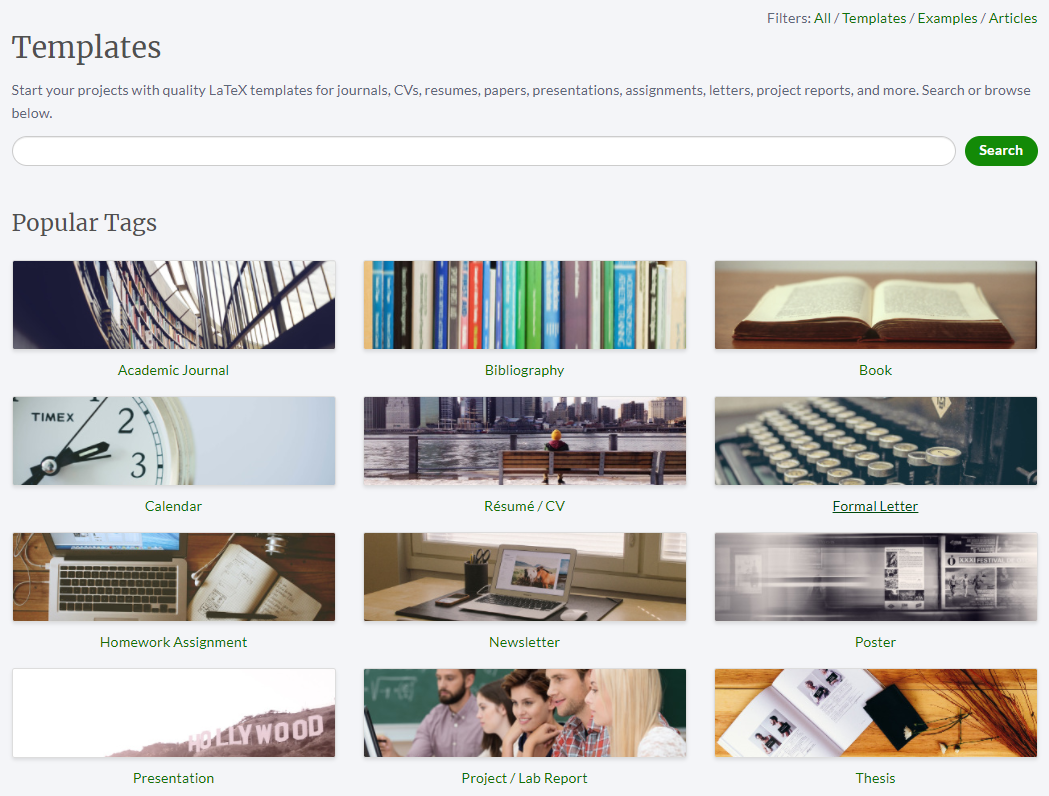
\includegraphics[width=0.7\linewidth]{day03-00-templates.png}
      \caption{Template categories on Overleaf.}
      \label{fig:day03-00-templates}
    \end{figure}
  \end{frame}
  }

  \nofoot{
  \begin{frame}{Templates}
    For academic journals, some official templates are available.
    \begin{figure}
      
\includegraphics[width=0.7\linewidth]{day03-01-official.png}
      \caption{Academic journal templates on Overleaf.}
      \label{fig:day03-01-official}
    \end{figure}
  \end{frame}
  }

  \nofoot{
  \begin{frame}{Uploading projects}
    Can also upload a \LaTeX \;project as a \texttt{.zip} file
    \begin{figure}
      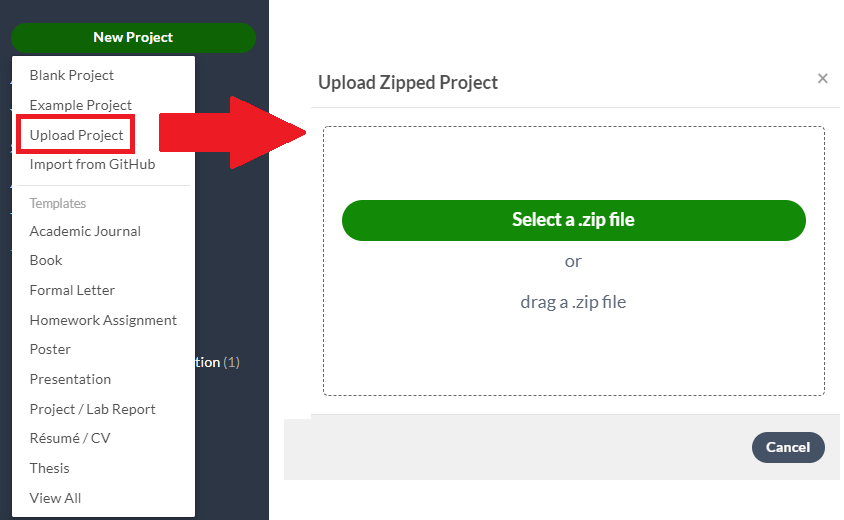
\includegraphics[width=0.7\linewidth]{day03-02-zip.png}
      \caption{``New Project'' $\rightarrow$ ``Upload project''.}
      \label{fig:day03-02-zip}
    \end{figure}
  \end{frame}
  }

  \section{CV/Resume Template}

  \begin{frame}[plain]
    \vfill
    \centering
    \begin{beamercolorbox}[sep=8pt,center,shadow=true,rounded=true]{CV/Resume Template}
      \usebeamerfont{title}\insertsectionhead\par%
      \color{davisblue}\noindent\rule{10cm}{1pt} \\
      % \footnotesize{}
    \end{beamercolorbox}
    \vfill
  \end{frame}

  \nofoot{
  \begin{frame}{Templates for Today} 
    Today, we'll work through a few templates.
    \begin{enumerate}
      \item Go to \texttt{https://github.com/mdelrosa/latex101/releases}
      \item Find the latest release
      \item Download \texttt{CV.zip} and \texttt{davis\_beamer\_template.zip}
    \end{enumerate}
    \begin{figure}
      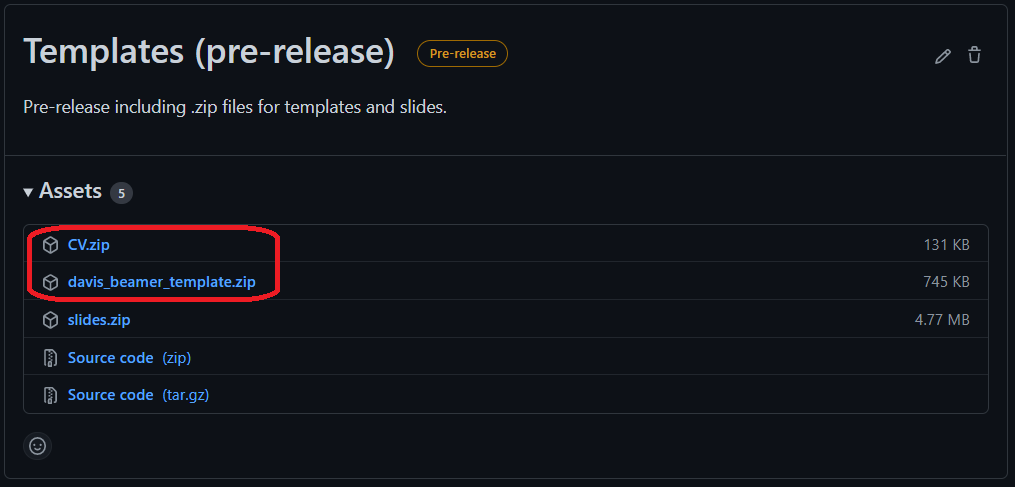
\includegraphics[width=0.7\linewidth]{day03-03-releases.png}
      \caption{\texttt{.zip} files for today's exercises.}
      \label{fig:day03-03-releases}
    \end{figure}
  \end{frame}
  }

  \nofoot{
  \begin{frame}{Uploading the CV project}
    Let's check out the CV project!
    \begin{figure}
      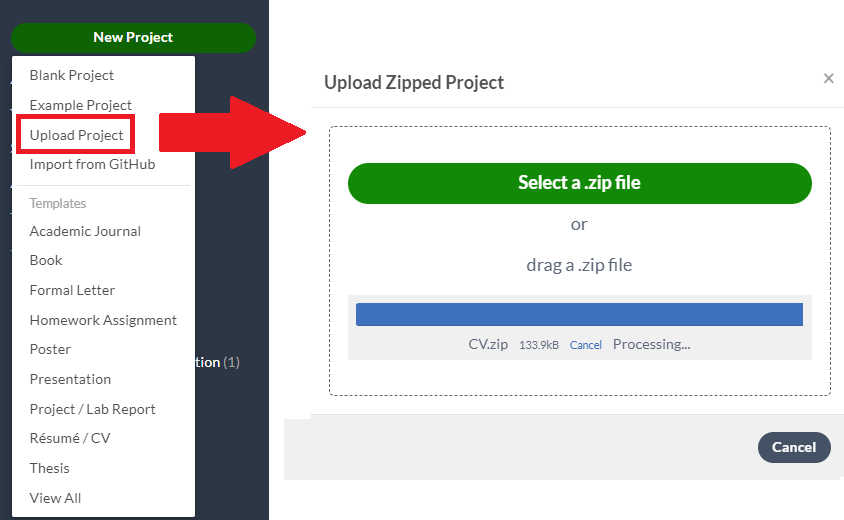
\includegraphics[width=0.7\linewidth]{day03-04-cvupload.png}
      \caption{Uploading our CV project.}
      \label{fig:day03-04-cvupload}
    \end{figure}
  \end{frame}
  }

  \nofoot{
  \begin{frame}{CV project}
    Project includes multiple files (\texttt{.tex}, \texttt{.cls})
    \begin{figure}
      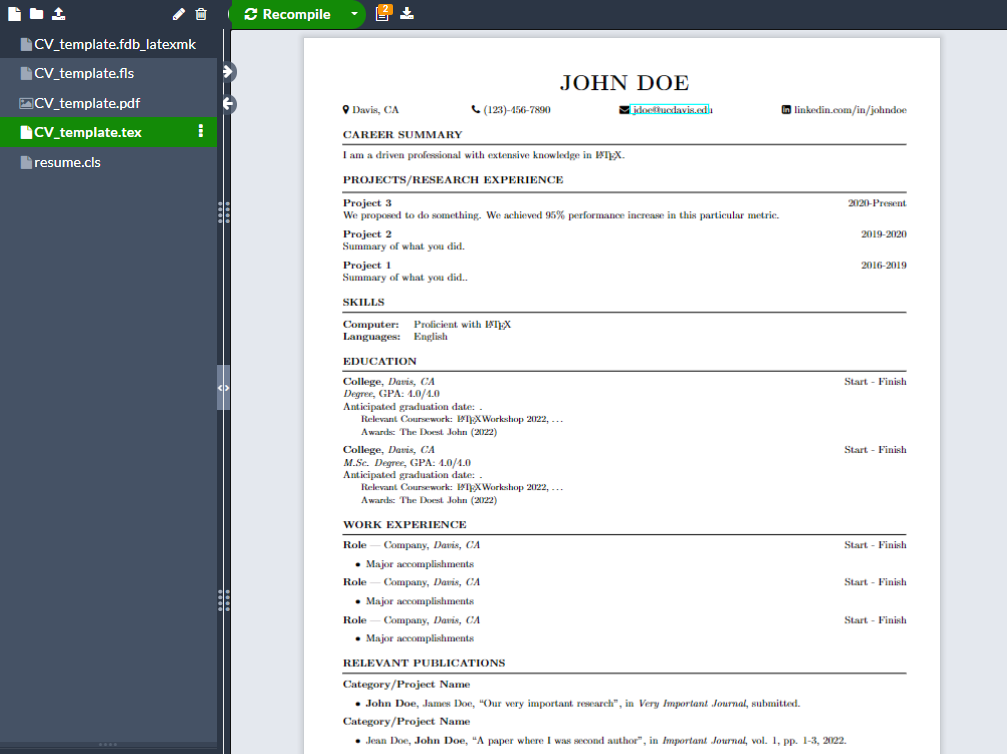
\includegraphics[width=\linewidth]{day03-05A-cvproject.png}
      \caption{CV project in Overleaf.}
      \label{fig:day03-05A-cvproject}
    \end{figure}
  \end{frame}
  }

  \nofoot{
  \begin{frame}{CV project: \texttt{.cls} file}
    \texttt{.cls} files define custom document classes.
    \begin{figure}
      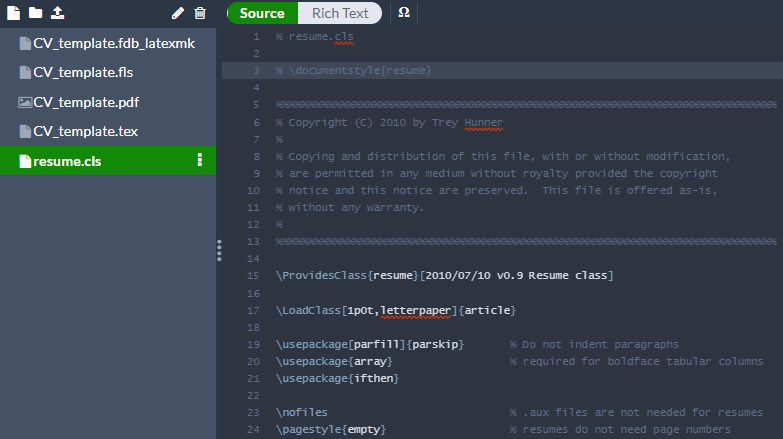
\includegraphics[width=\linewidth]{day03-05B-cvcls.png}
      \caption{The \texttt{resume.cls} file in the CV project.}
      \label{fig:day03-05B-cvcls}
    \end{figure}
  \end{frame}
  }

  \nofoot{
  \begin{frame}{CV project: \texttt{\textbackslash documentclass}}
    \texttt{\textbackslash documentclass} imports the custom class from the \texttt{.cls} file.
    \begin{figure}
      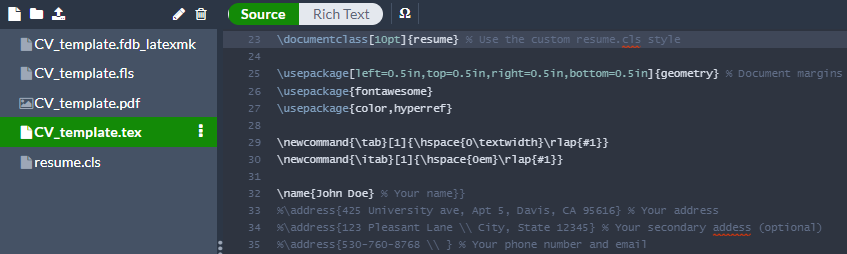
\includegraphics[width=\linewidth]{day03-05C-cvdocclass.png}
      \caption{Importing \texttt{resume} from \texttt{resume.cls}.}
      \label{fig:day03-05C-cvdocclass}
    \end{figure}
  \end{frame}
  }

  \nofoot{
  \begin{frame}{CV project: Header}
    \begin{itemize}
      \item \texttt{\textbackslash fa} commands define icons.
      \item \texttt{\textbackslash hfill} creates horizontal whitespace to fill current line
    \end{itemize}
    \begin{figure}
      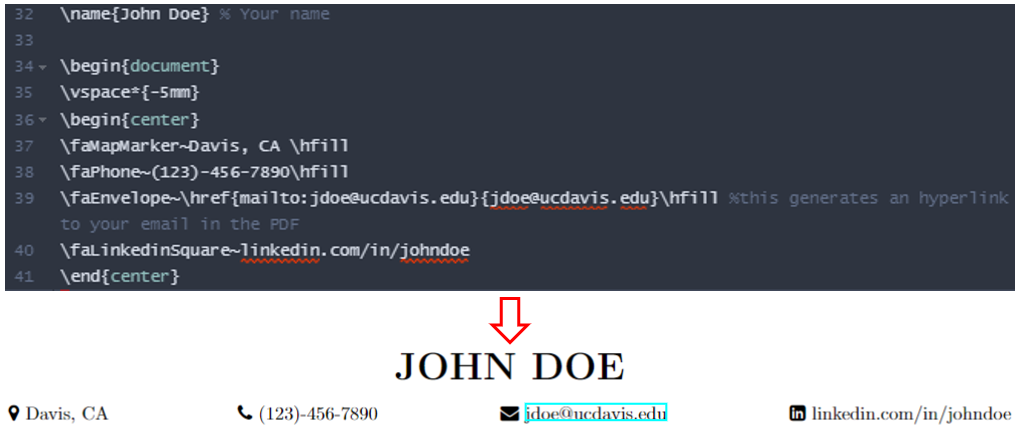
\includegraphics[width=\linewidth]{day03-05D-cvaddress.png}
      \caption{CV header with icons for contact information.}
      \label{fig:day03-05D-cvaddress}
    \end{figure}
  \end{frame}
  }

  \nofoot{
  \begin{frame}{CV project: Summary}
    \begin{itemize}
      \item \texttt{\textbackslash rSection}: custom \texttt{Section} environment.
    \end{itemize}
    \begin{figure}
      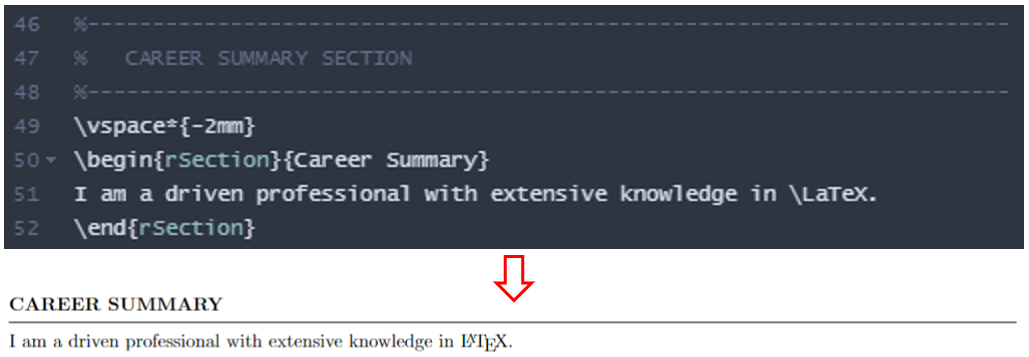
\includegraphics[width=\linewidth]{day03-05E-cvsummary.png}
      \caption{CV summary with an \texttt{rSection} environment.}
      \label{fig:day03-05E-cvsummary}
    \end{figure}
  \end{frame}
  }

  \nofoot{
  \begin{frame}{CV project: Projects/Research}
    \begin{figure}
      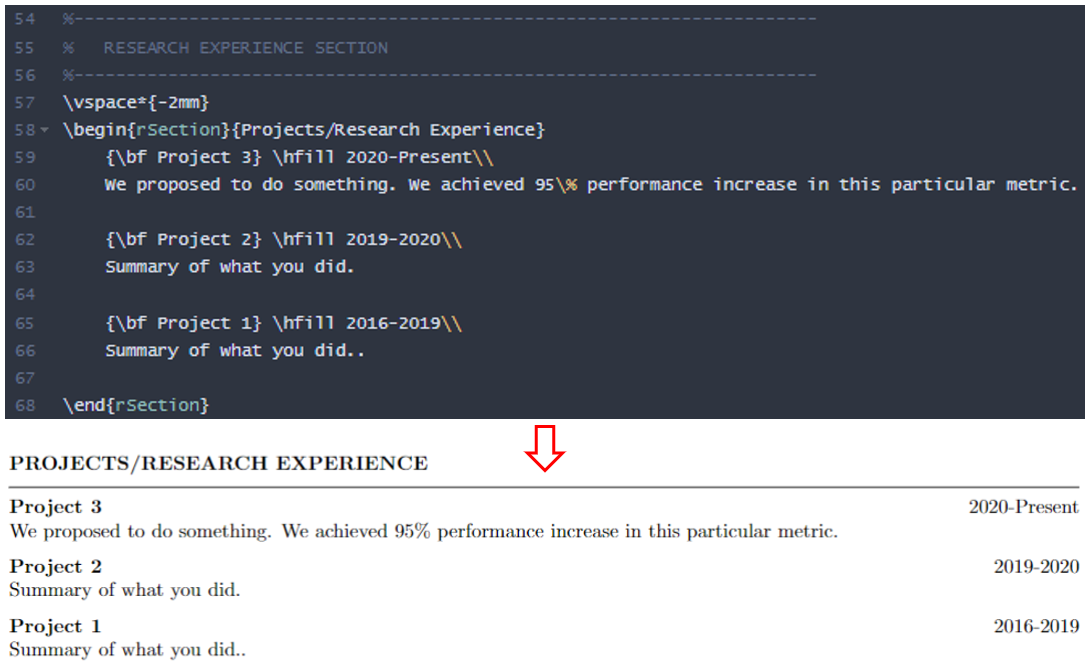
\includegraphics[width=\linewidth]{day03-05F-cvresearch.png}
      \caption{CV \texttt{rSection} for projects/research.}
      \label{fig:day03-05F-cvresearch}
    \end{figure}
  \end{frame}
  }

  \nofoot{
  \begin{frame}{CV project: Skills}
    \begin{itemize}
      \item \texttt{@\{text\}}: Inserts `text' in every row.
      \item \texttt{$>$\{\textbackslash bfseries\}}: Applies bold face to entire column.
      \item \texttt{\textbackslash hspace\{3ex\}}: \texttt{ex} denotes horizontal size of `x' in the given font.
    \end{itemize}
    \begin{figure}
      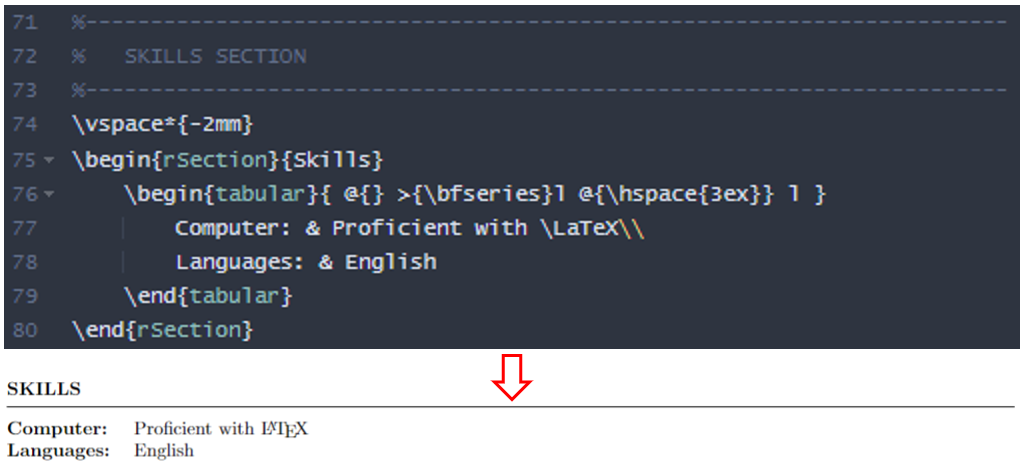
\includegraphics[width=\linewidth]{day03-05G-cvskills.png}
      \caption{CV \texttt{rSection} for skills.}
      \label{fig:day03-05G-cvskills}
    \end{figure}
  \end{frame}
  }

  \nofoot{
  \begin{frame}{CV project: Education}
    \begin{figure}
      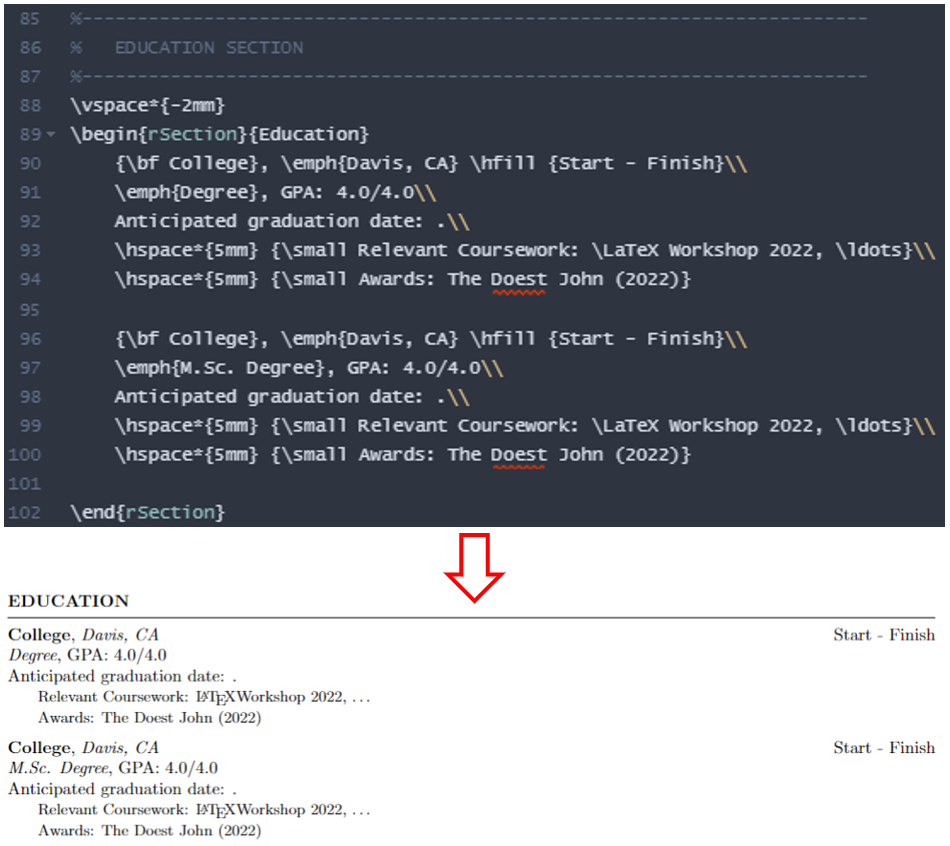
\includegraphics[width=0.7\linewidth]{day03-05H-cvedu.png}
      \caption{CV \texttt{rSection} for education.}
      \label{fig:day03-05H-cvedu}
    \end{figure}
  \end{frame}
  }

  \nofoot{
  \begin{frame}{CV project: Work Experience}
    \begin{figure}
      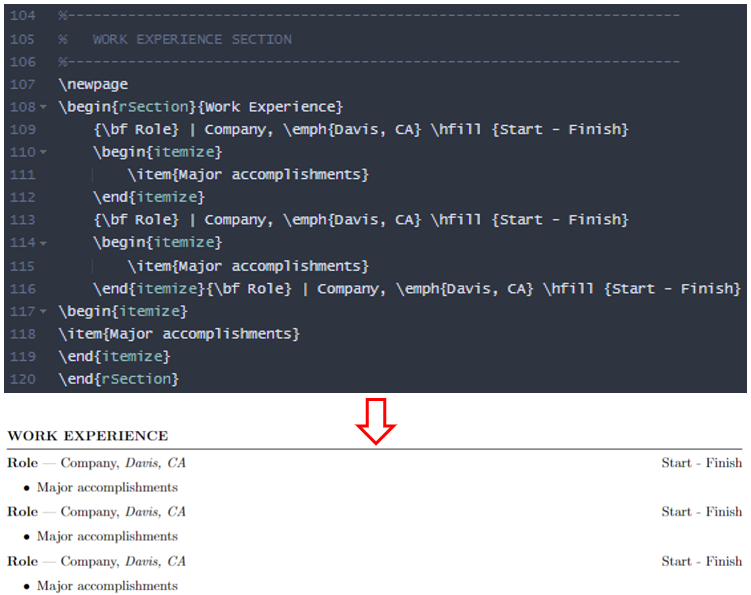
\includegraphics[width=0.7\linewidth]{day03-05I-cvwork.png}
      \caption{CV \texttt{rSection} for work experience.}
      \label{fig:day03-05I-cvwork}
    \end{figure}
  \end{frame}
  }

  \nofoot{
  \begin{frame}{CV project: Publications}
    \begin{figure}
      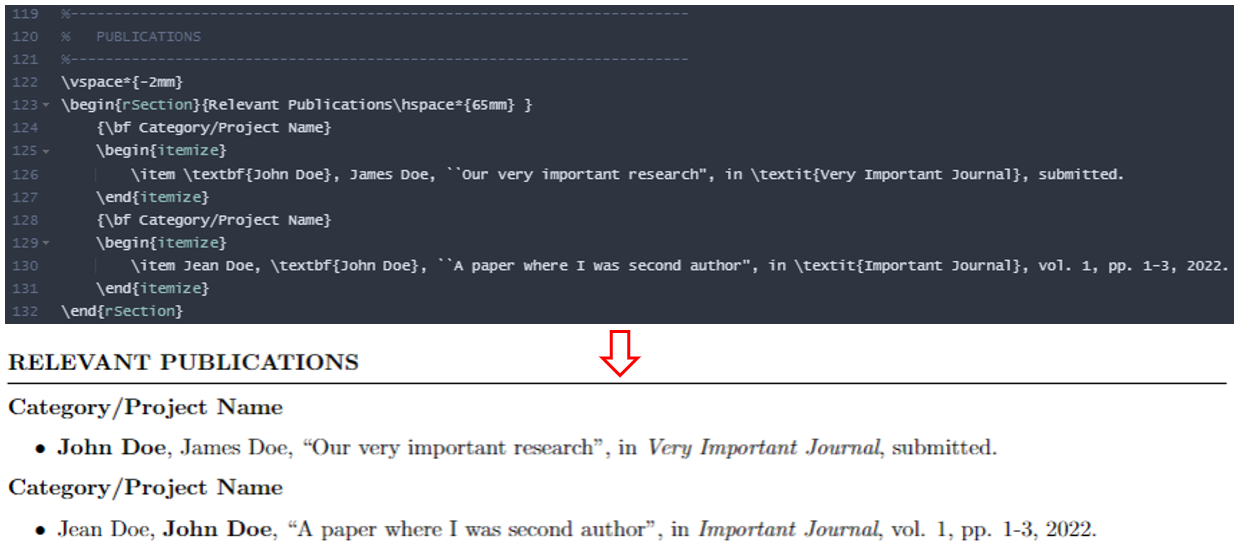
\includegraphics[width=0.9\linewidth]{day03-05J-cvpub.png}
      \caption{CV \texttt{rSection} for publications.}
      \label{fig:day03-05I-cvpub}
    \end{figure}
  \end{frame}
  }

  \section{Beamer Template}

  \begin{frame}[plain]
    \vfill
    \centering
    \begin{beamercolorbox}[sep=8pt,center,shadow=true,rounded=true]{Beamer Templates}
      \usebeamerfont{title}\insertsectionhead\par%
      \color{davisblue}\noindent\rule{10cm}{1pt} \\
      \footnotesize{Slide decks for academic presentations.}
    \end{beamercolorbox}
    \vfill
  \end{frame}

\begin{frame}{End of Day 3}
  \begin{itemize}
    \item Lessons 1-12 from \texttt{learnlatex.org}
    \item Today: Templates (Resume/CV, Beamer)
  \end{itemize}
\end{frame}

\begin{frame}{References}
  \bibliographystyle{ieeetr}
  \bibliography{example}
\end{frame}

} %end footnotsize

\end{document}
